% =====================================================================
%  CAPÍTULO 4 — Ejemplo: discusión (subfiguras y listas)
% =====================================================================
\chapter{Título del capítulo 4}\label{cap:capitulo4}

\section{Introducción del capítulo}

\lipsum[13]

\section{Análisis}

La \cref{fig:paneles} compara \ldots: el panel~\subref{fig:panel-a} \ldots
y el panel~\subref{fig:panel-b} \ldots

\begin{figure}[htbp]
  \centering
  \begin{subfigure}{0.48\textwidth}
    \centering
    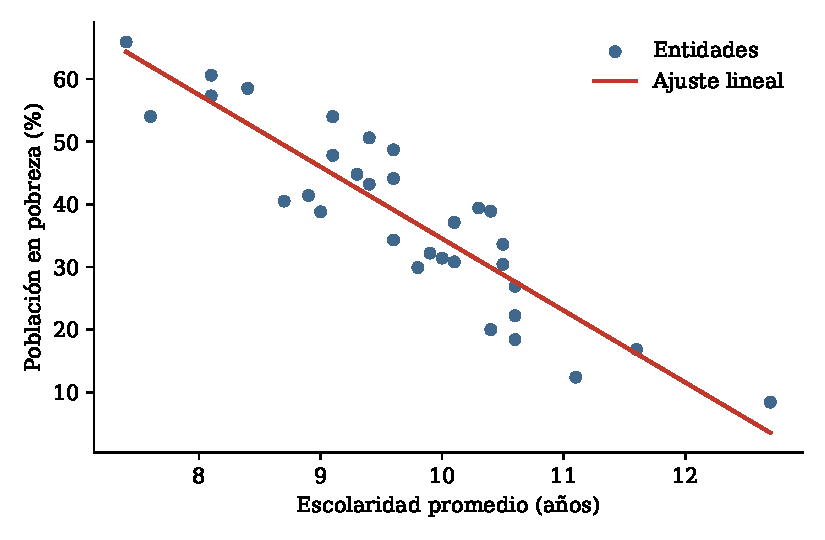
\includegraphics[width=\linewidth]{figura_ejemplo}
    \caption{Panel A}\label{fig:panel-a}
  \end{subfigure}\hfill
  \begin{subfigure}{0.48\textwidth}
    \centering
    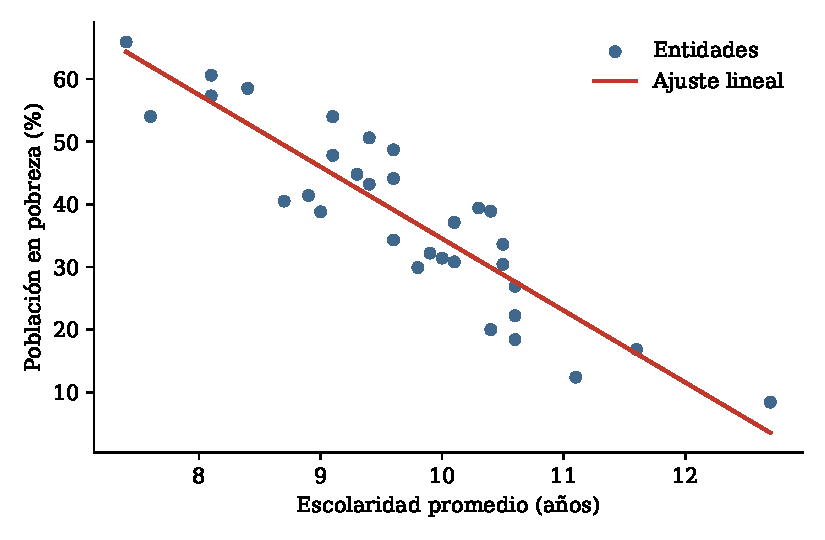
\includegraphics[width=\linewidth]{figura_ejemplo}
    \caption{Panel B}\label{fig:panel-b}
  \end{subfigure}
  \caption{Figura con dos paneles}
  \label{fig:paneles}
\end{figure}

\section{Discusión}

Los hallazgos principales son:
\begin{itemize}
  \item \lipsum[14][1-2]
  \item \lipsum[14][3-4]
  \item \lipsum[14][5-6]
\end{itemize}

\lipsum[15]
